\documentclass[10pt,a4paper,headinclude,footinclude,hidelinks]{scrreprt} % KOMA-Script
\usepackage[italian]{babel}
\usepackage[utf8]{inputenc}
\usepackage[T1]{fontenc}
\usepackage{graphicx}
\usepackage{amsfonts}
\usepackage[]{../../classicthesis} % nochapters
\pagestyle{scrheadings}
\setcounter{tocdepth}{1}

\begin{document}
    \title{\rmfamily\normalfont\spacedallcaps{Analisi dei requisiti}}
    \author{\spacedlowsmallcaps{Nicola Moretto (matr. 578258)}}
    \date{\today}
    
    \maketitle
    
    \begin{abstract}
        \noindent Il documento illustra i casi d'uso e i requisiti dell'interfaccia grafica per la visualizzazione e la navigazione dei contenuti.
    \end{abstract}
    
	\begin{table}[ht]
	\centering
	\begin{tabular}{|c|c|l|}
	\hline
	\textsc{Versione} & \textsc{Data} & \textsc{Modifiche} \\ \hline
	0.1 & 8-10-2012 & Stesura iniziale del documento. \\ \hline
	0.2 & 10-10-2012 & Redatte le sezioni \ref{ch:stage:ar:uc:1} e \ref{ch:stage:ar:uc:2}. \\ \hline
	0.3 & 11-10-2012 & Ampliata e rivista la sezione \ref{ch:stage:ar:uc:2}. \\ \hline
	0.4 & 11-10-2012 & Redatte le sezioni \ref{ch:stage:ar:uc:3} e \ref{ch:stage:ar:uc:4}. \\ \hline
	0.5 & 12-10-2012 & Redatti i capitoli \ref{ch:stage:ar:intro} e \ref{ch:stage:ar:requisiti}. \\ \hline
	0.6 & 13-10-2012 & Aggiunti i diagrammi UML dei casi d'uso. \\ \hline
	\end{tabular}
	\caption{Registro delle modifiche}
	\label{tab:stage:wp:workload}
	\end{table}

	\tableofcontents

	\listoffigures

	%----------
	% CAPITOLO
	%----------
	\chapter{Introduzione}
	\label{ch:stage:ar:intro}

	\section{Presentazione del prodotto}
	\label{sec:stage:ar:intro:presentazione}
	Il prodotto consiste in un'interfaccia grafica per la consultazione dei risultati di ricerche sui contenuti informativi pubblicati nella piattaforma web tematica \textit{Social (Life) Shuttle}.

	Si tratta di una componente software destinata ad essere integrata all'interno di una piattaforma web esistente, nell'ambito della quale sono definiti (a livello di interfaccia o implementazione) i contenuti, i sistemi di classificazione e le componenti con cui essa è chiamata ad interagire.

	\section{Scopo del prodotto}
	\label{sec:stage:ar:intro:scopo}
	Lo scopo del prodotto consiste nell'offrire un'interfaccia grafica innovativa ed intuitiva, che faciliti la consultazione dei risultati di una ricerca tra i contenuti pubblicati dagli utenti sulla piattaforma.

	Tale interfaccia deve fornire una rappresentazione - grafica e/o testuale - efficace delle informazioni fondamentali di ciascun contenuto e dei legami reciproci, oltre ad offrire strumenti opportuni per raffinare i risultati di ricerca, agendo sui criteri di classificazione (argomento, emozione, etichetta, giudizio, intenzione) e le proprietà di ciascun contenuto (autore, data di pubblicazione, \ldots).

	Il prodotto deve permettere inoltre un'agevole consultazione delle discussioni, ossia i flussi di contenuti pubblicati dagli utenti in risposta - diretta o indiretta - a ciascun contenuto specifico.

	\section{Vincoli del prodotto}
	\label{sec:stage:ar:intro:vincoli}
	L'interfaccia grafica deve risultare usabile e fruibile in contesti caratterizzati da un elevato numero di contenuti restituiti da una ricerca o dall'impiego di dispositivi aventi caratteristiche limitate (risoluzione, potenza di calcolo, dimensione dello schermo, \ldots).

	\section{Caratteristiche degli utenti}
	\label{sec:stage:ar:intro:utenti}
	Il prodotto software dev'essere utilizzabile facilmente da qualsiasi utente, a prescindere dalle competenze in suo possesso e dalla familiarità con piattaforme web tematiche esistenti, e fruibile dalla maggior varietà possibile di dispositivi.

	Ciascun utente registrato alla piattaforma, cui sono associati un profilo esperienziale e una serie di interessi, dovrebbe beneficiare di ulteriori vantaggi, consistenti nella possibilità di filtrare automaticamente i risultati di ricerca coerenti con il proprio profilo e gli interessi dichiarati.

	\section{Riferimenti informativi}
	\label{sec:stage:ar:intro:riferimenti}

	\begin{itemize}
	\item Tracciamento dei requisiti (\textit{tracciamento.ods} allegato alla presente documentazione).
	\end{itemize}

	\chapter{Casi d'uso}
	\label{ch:stage:ar:uc}

	\section{UC.1 - Ricerca di contenuti informativi}
	\label{ch:stage:ar:uc:1}

	\begin{figure}[ht]
		\begin{center}
	    	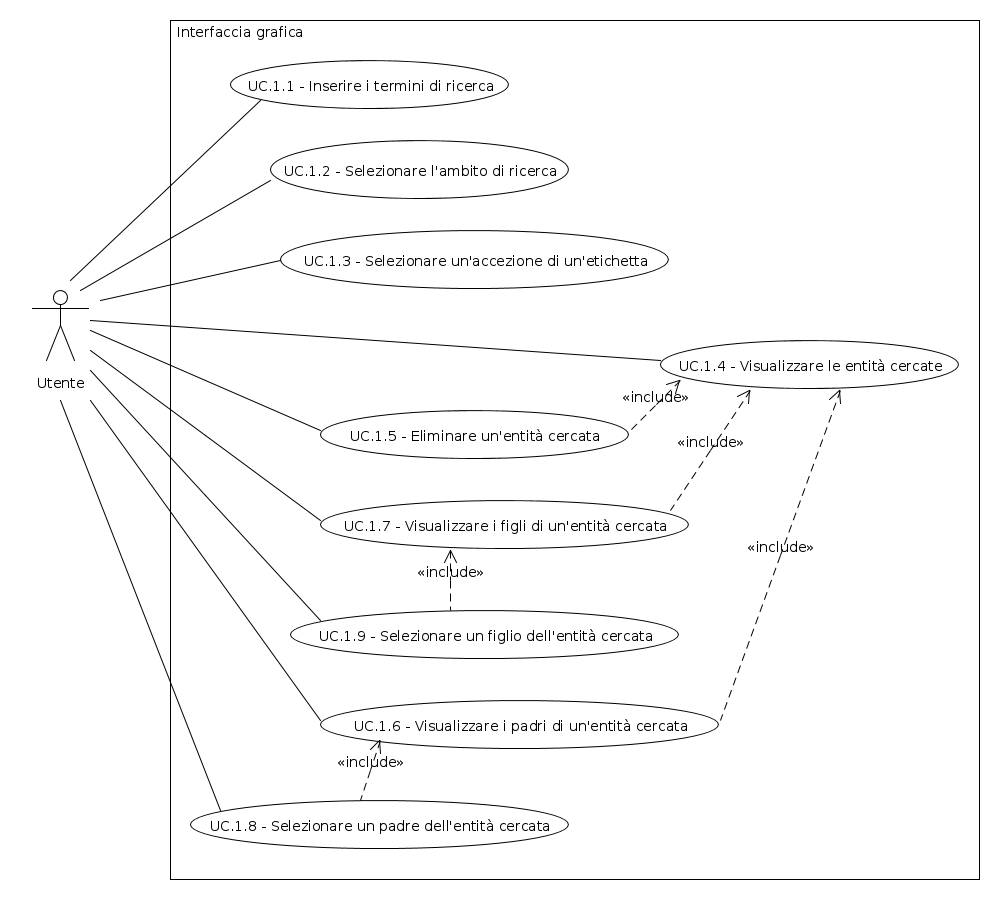
\includegraphics[width=12cm]{uc_1.png}
			\label{gfx:uc:1}
			\caption{UC.1 - Ricerca di contenuti informativi}
		\end{center}
	\end{figure}

	Il diagramma dei casi d'uso (v. figura \ldots) descrive l'interazione dell'utente per eseguire una ricerca sui contenuti pubblicati nella piattaforma.

	Il primo passo\marginpar{Criteri di ricerca} consiste nell'inserire le chiavi di ricerca (\nameref{sec:stage:ar:uc:1_1}), che possono rappresentare etichette del dizionario assegnate ai contenuti o frasi citate all'interno di questi ultimi, nel titolo o nel corpo: l'utente può quindi restringere l'ambito di ricerca alle sole etichette o frasi (\nameref{sec:stage:ar:uc:1_2}).

	Per ogni etichetta\marginpar{Etichette ed accezioni} inserita, ove essa possieda accezioni multiple, l'utente è chiamato a indicare quelle di interesse (\nameref{sec:stage:ar:uc:1_3}): nel complesso, esse individuano un insieme di entità di cui si desiderano ottenere informazioni.

	I risultati di ricerca riportano la lista delle entità cercate (\nameref{sec:stage:ar:uc:1_4}), che l'utente può modificare - per alterare i criteri di ricerca - eliminando un'entità (\nameref{sec:stage:ar:uc:1_5}) oppure sostituendola con un'entità padre (\nameref{sec:stage:ar:uc:1_6}) o figlio (\nameref{sec:stage:ar:uc:1_7}).

 	\subsection[UC.1.1]{UC.1.1 - Inserire i termini di ricerca}
	\label{sec:stage:ar:uc:1_1}
	\paragraph{Attori:}  utente
	\paragraph{Precondizioni:} il browser visualizza la pagina di ricerca.
	\paragraph{Postcondizioni:} la barra di ricerca contiene una lista di stringhe separate da virgole.
	\paragraph{Scenario principale} \hfill \\
	L'utente inserisce i termini o le espressioni, separati da virgola, nella barra di ricerca, potendo avvantaggiarsi - per le etichette - di un meccanismo di completamento automatico durante la digitazione.

	\subsection[UC.1.2]{UC.1.2 - Selezionare l'ambito di ricerca}
	\label{sec:stage:ar:uc:1_2}
	\paragraph{Attori:} utente
	\paragraph{Precondizioni:} il browser visualizza la pagina di ricerca.
	\paragraph{Postcondizioni:} l'utente ha impostato l'ambito di ricerca desiderato.
	\paragraph{Scenario principale} \hfill \\
	L'utente seleziona uno dei possibili ambiti in cui effettuare la ricerca:
	\begin{itemize}
	\item solo etichette;
	\item solo frasi;
	\item etichette e frasi (predefinito).
	\end{itemize}

	\subsection[UC.1.3]{UC.1.3 - Selezionare un'accezione di un'etichetta}
	\label{sec:stage:ar:uc:1_3}
	\paragraph{Attori:} utente
	\paragraph{Precondizioni:} il sistema mostra un elenco di accezioni relative ad un'etichetta inserita come termine di ricerca.
	\paragraph{Postcondizioni:} il sistema ha associato un'entità precisa all'etichetta.
	\paragraph{Scenario principale}  \hfill \\
	L'utente seleziona l'accezione dell'etichetta facente riferimento all'entità intesa.

	\subsection[UC.1.4]{UC.1.4 - Visualizzare le entità cercate}
	\label{sec:stage:ar:uc:1_4}
	\paragraph{Attori:} utente
	\paragraph{Precondizioni:} il sistema mostra i risultati della ricerca.
	\paragraph{Postcondizioni:} il sistema mostra le entità cercate nei contenuti .
	\paragraph{Scenario principale} \hfill \\
	In un'area dedicata l'utente visualizza la lista delle entità cercate nei contenuti e riferite dalle etichette inserite come termini di ricerca (o dalle relative accezioni).

	\subsection[UC.1.5]{UC.1.5 - Eliminare un'entità cercata}
	\label{sec:stage:ar:uc:1_5}
	\paragraph{Attori:} utente
	\paragraph{Precondizioni:} il sistema mostra la lista delle entità cercate nei contenuti.
	\paragraph{Postcondizioni:} un'entità è stata eliminata dalla lista e i risultati di ricerca sono stati aggiornati.
	\paragraph{Scenario principale}
	\begin{enumerate}
	\item L'utente visualizza la lista delle entità (\nameref{sec:stage:ar:uc:1_4});
	\item l'utente seleziona un'entità;
	\item l'utente cancella l'entità dalla lista.
	\end{enumerate}
	\paragraph{Scenari alternativi}
	\begin{enumerate}
	\item l'entità cercata non è presente nella lista
		\begin{enumerate}
		\item l'utente non effettua alcuna operazione.
		\end{enumerate}
	\end{enumerate}

	\subsection[UC.1.6]{UC.1.6 - Visualizzare i padri di un'entità cercata}
	\label{sec:stage:ar:uc:1_6}
	\paragraph{Attori:} utente
	\paragraph{Precondizioni:} il sistema mostra la lista delle entità cercate nei contenuti.
	\paragraph{Postcondizioni:} il sistema visualizza l'insieme dei padri di un'entità presente nella lista.
	\paragraph{Scenario principale}
	\begin{enumerate}
	\item L'utente visualizza la lista delle entità (\nameref{sec:stage:ar:uc:1_4});
	\item l'utente seleziona un'entità;
	\item l'utente richiama la lista delle entità padre.
	\end{enumerate}

	\subsection[UC.1.7]{UC.1.7 - Visualizzare i figli di un'entità cercata}
	\label{sec:stage:ar:uc:1_7}
	\paragraph{Attori:} utente
	\paragraph{Precondizioni:} il sistema mostra la lista delle entità cercate nei contenuti.
	\paragraph{Postcondizioni:} il sistema visualizza l'insieme dei figli di un'entità presente nella lista.
	\paragraph{Scenario principale}
	\begin{enumerate}
	\item L'utente visualizza la lista delle entità (\nameref{sec:stage:ar:uc:1_4});
	\item l'utente seleziona un'entità;
	\item l'utente richiama la lista delle entità figlie.
	\end{enumerate}

	\subsection[UC.1.8]{UC.1.8 - Selezionare un padre dell'entità cercata}
	\label{sec:stage:ar:uc:1_8}
	\paragraph{Attori:} utente
	\paragraph{Precondizioni:} il sistema mostra la lista delle entità cercate nei contenuti.
	\paragraph{Postcondizioni:} un'entità è stata sostituita con un padre e i risultati di ricerca sono stati aggiornati.
	\paragraph{Scenario principale}
	\begin{enumerate}
	\item L'utente richiama la lista dei padri di un'entità (\nameref{sec:stage:ar:uc:1_6});
	\item l'utente seleziona un'entità padre.
	\end{enumerate}

	\subsection[UC.1.9]{UC.1.9 - Selezionare un figlio dell'entità cercata}
	\label{sec:stage:ar:uc:1_9}
	\paragraph{Attori:} utente
	\paragraph{Precondizioni:} il sistema mostra la lista delle entità cercate nei contenuti.
	\paragraph{Postcondizioni:} un'entità è stata sostituita con un figlio e i risultati di ricerca sono stati aggiornati.
	\paragraph{Scenario principale}
	\begin{enumerate}
	\item L'utente richiama la lista dei figli di un'entità (\nameref{sec:stage:ar:uc:1_7});
	\item l'utente seleziona un'entità figlia.
	\end{enumerate}

	% SECTION
	\section{UC.2 - Raffinamento dei criteri di ricerca}
	\label{ch:stage:ar:uc:2}

	\begin{figure}[]
		\begin{center}
	    	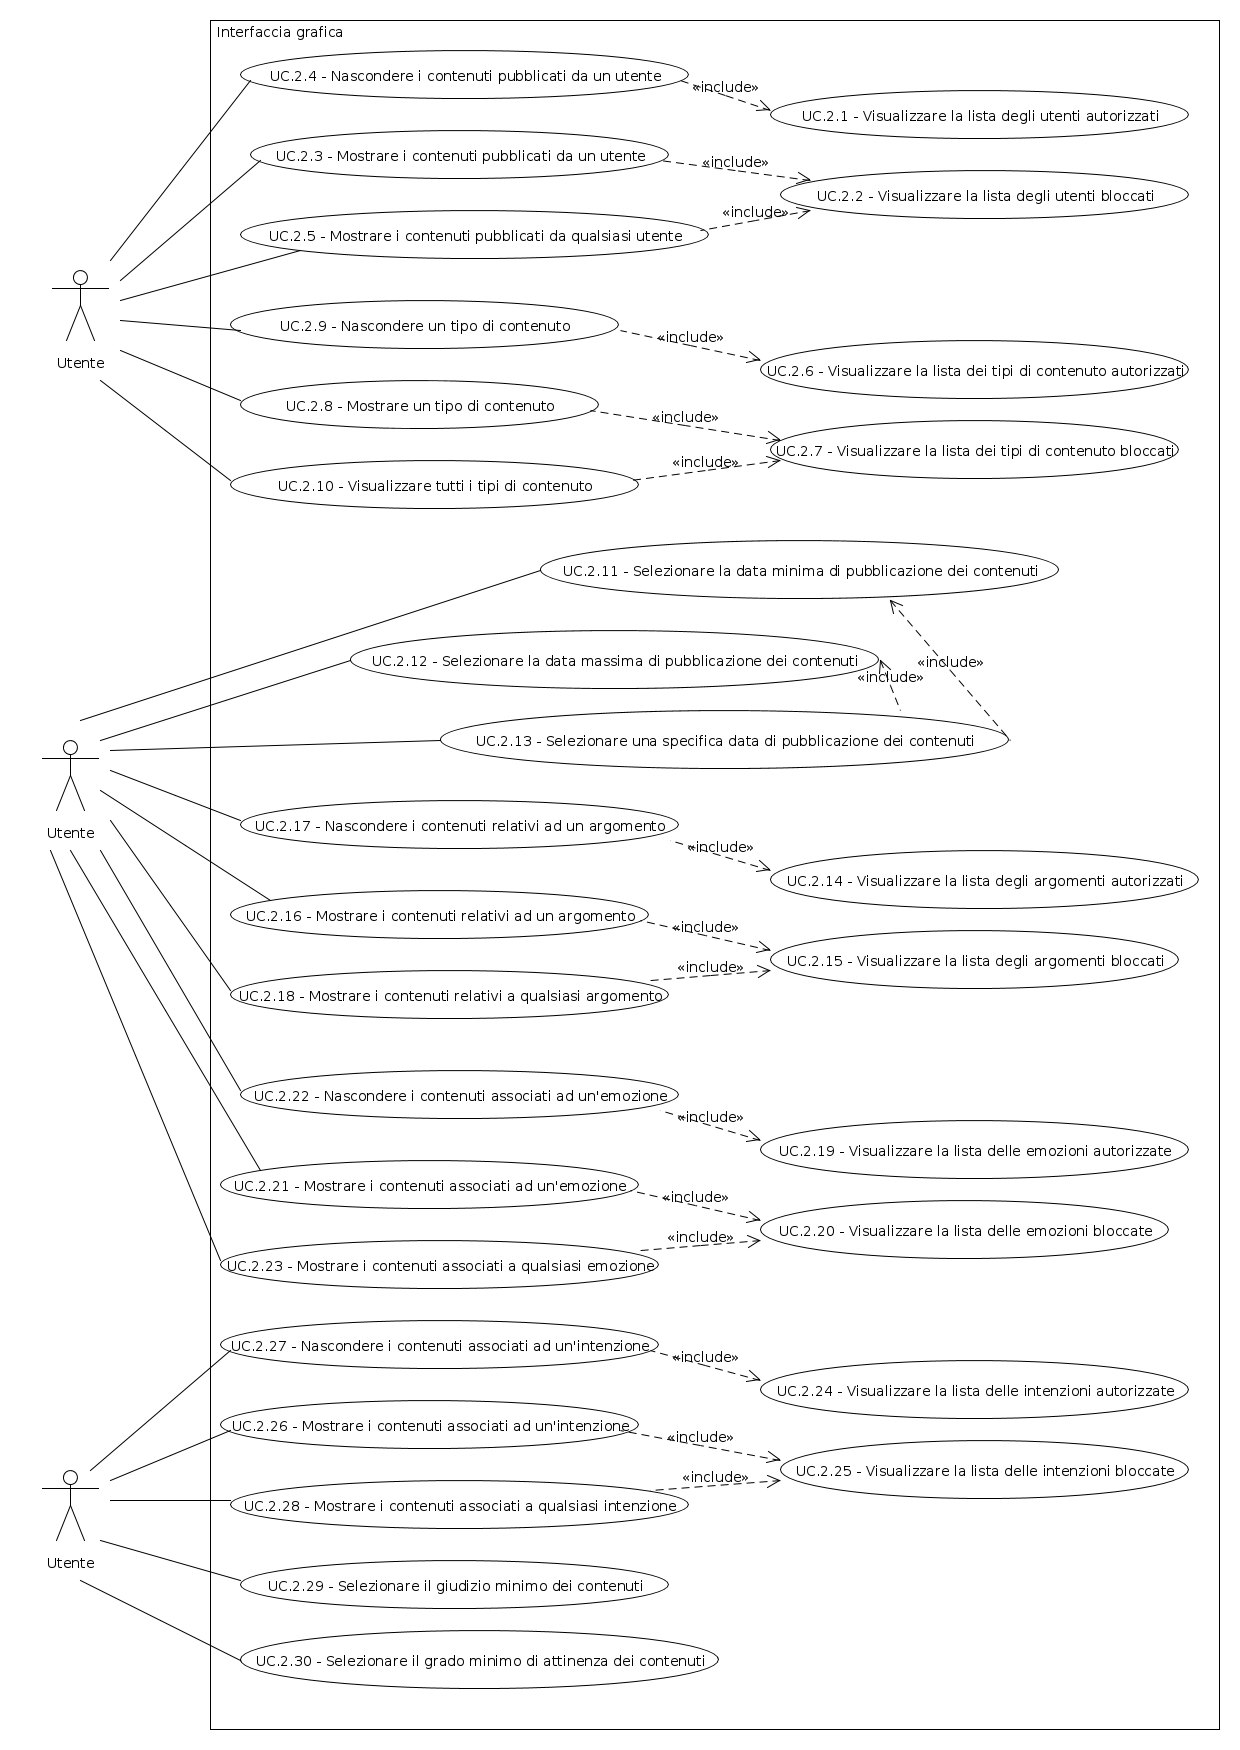
\includegraphics[width=12cm]{uc_2.png}
			\label{gfx:uc:2}
			\caption{UC.2 - Raffinamento dei criteri di ricerca}
		\end{center}
	\end{figure}

	Questo diagramma dei casi d'uso (vedi \ldots) mostra le possibilità offerte all'utente per raffinare i criteri di ricerca così da ridurre la dimensione e migliorare la qualità e l'attinenza dei risultati di ricerca.

	L'utente può intervenire su un'ampia varietà di parametri, suddivisi tra criteri di classificazione e proprietà dei contenuti.

	\paragraph{Criteri di classificazione}
	\begin{itemize}
	\item argomento;
	\item emozione;
	\item giudizio;
	\item intenzione.
	\end{itemize}

	\paragraph{Propriet\`a}
	\begin{itemize}
	\item autore;
	\item data di pubblicazione;
	\item tipo.
	\end{itemize}

	\subsection[UC.2.1]{UC.2.1 - Visualizzare la lista degli utenti autorizzati}
	\label{sec:stage:ar:uc:2_1}
	\paragraph{Attori:} utente
	\paragraph{Precondizioni:} il sistema visualizza i contenuti corrispondenti ai criteri di ricerca immessi e ai filtri impostati.
	\paragraph{Postcondizioni:} il sistema mostra la lista degli utenti autorizzati, ossia aventi pubblicato almeno un contenuto presente e visualizzato tra i risultati di ricerca.
	\paragraph{Scenario principale}
	L'utente apre la lista degli utenti autorizzati.

	\subsection[UC.2.2]{UC.2.2 - Visualizzare la lista degli utenti bloccati}
	\label{sec:stage:ar:uc:2_2}
	\paragraph{Attori:} utente
	\paragraph{Precondizioni:} il sistema visualizza i contenuti corrispondenti ai criteri di ricerca immessi e ai filtri impostati.
	\paragraph{Postcondizioni:} il sistema mostra la lista degli utenti bloccati, ossia aventi pubblicato almeno un contenuto presente ma non visualizzato tra i risultati di ricerca.
	\paragraph{Scenario principale} \hfill \\
	L'utente apre la lista degli utenti bloccati.

	\subsection[UC.2.3]{UC.2.3 - Mostrare i contenuti pubblicati da un utente}
	\label{sec:stage:ar:uc:2_3}
	\paragraph{Attori:} utente
	\paragraph{Precondizioni:} il sistema visualizza i contenuti corrispondenti ai criteri di ricerca immessi e ai filtri impostati.
	\paragraph{Postcondizioni:} il sistema mostra - in aggiunta ai precedenti - i contenuti pubblicati dall'utente selezionato e corrispondenti ai criteri di ricerca.
	\paragraph{Scenario principale}
	\begin{enumerate}
	\item l'utente visualizza la lista degli utenti bloccati (\nameref{sec:stage:ar:uc:2_2});
	\item l'utente seleziona quello di cui desidera visualizzare i contenuti tra i risultati di ricerca;
	\item l'utente lo sposta nella lista degli utenti autorizzati.
	\end{enumerate}

	\subsection[UC.2.4]{UC.2.4 - Nascondere i contenuti pubblicati da un utente}
	\label{sec:stage:ar:uc:2_4}
	\paragraph{Attori:} utente
	\paragraph{Precondizioni:} il sistema visualizza i contenuti corrispondenti ai criteri di ricerca immessi e ai filtri impostati.
	\paragraph{Postcondizioni:} il sistema nasconde dai risultati di ricerca i contenuti pubblicati dall'utente selezionato.
	\paragraph{Scenario principale}
	\begin{enumerate}
	\item l'utente visualizza la lista degli utenti autorizzati (\nameref{sec:stage:ar:uc:2_1});
	\item l'utente seleziona quello di cui desidera nascondere i contenuti presenti nei risultati di ricerca;
	\item l'utente lo sposta nella lista degli utenti bloccati.
	\end{enumerate}

	\subsection[UC.2.5]{UC.2.5 - Mostrare i contenuti pubblicati da qualsiasi utente}
	\label{sec:stage:ar:uc:2_5}
	\paragraph{Attori:} utente
	\paragraph{Precondizioni:} il sistema visualizza i contenuti corrispondenti ai criteri di ricerca immessi e ai filtri impostati.
	\paragraph{Postcondizioni:} il sistema mostra i contenuti corrispondenti ai criteri immessi e ai filtri impostati, a prescindere dall'utente che li ha pubblicati.
	\paragraph{Scenario principale}
	\begin{enumerate}
	\item l'utente visualizza la lista degli utenti bloccati (\nameref{sec:stage:ar:uc:2_2});
	\item l'utente svuota la lista.
	\end{enumerate}

	\subsection[UC.2.6]{UC.2.6 - Visualizzare la lista dei tipi di contenuto autorizzati}
	\label{sec:stage:ar:uc:2_6}
	\paragraph{Attori:} utente
	\paragraph{Precondizioni:} il sistema visualizza i contenuti corrispondenti ai criteri di ricerca immessi e ai filtri impostati.
	\paragraph{Postcondizioni:} il sistema mostra la lista dei tipi di contenuto autorizzati, ossia visualizzati tra i risultati di ricerca.
	\paragraph{Scenario principale} \hfill \\
	L'utente apre la lista dei tipi di contenuto autorizzati.

	\subsection[UC.2.7]{UC.2.7 - Visualizzare la lista dei tipi di contenuto bloccati}
	\label{sec:stage:ar:uc:2_7}
	\paragraph{Attori:} utente
	\paragraph{Precondizioni:} il sistema visualizza i contenuti corrispondenti ai criteri di ricerca immessi e ai filtri impostati.
	\paragraph{Postcondizioni:} il sistema mostra la lista dei tipi di contenuto bloccati, ossia rimossi dai risultati di ricerca.
	\paragraph{Scenario principale} \hfill \\
	L'utente apre la lista dei tipi di contenuto bloccati.

	\subsection[UC.2.8]{UC.2.8 - Mostrare un tipo di contenuto}
	\label{sec:stage:ar:uc:2_8}
	\paragraph{Attori:} utente
	\paragraph{Precondizioni:} il sistema visualizza i contenuti corrispondenti ai criteri di ricerca immessi e ai filtri impostati.
	\paragraph{Postcondizioni:} il sistema mostra - in aggiunta ai precedenti - i contenuti corrispondenti al tipo selezionato e ai criteri di ricerca.
	\paragraph{Scenario principale}
	\begin{enumerate}
	\item l'utente visualizza la lista dei tipi di contenuto bloccati (\nameref{sec:stage:ar:uc:2_7});
	\item l'utente seleziona il tipo di contenuto che desidera visualizzare tra i risultati di ricerca;
	\item l'utente lo sposta nella lista dei tipi di contenuto autorizzati.
	\end{enumerate}

	\subsection[UC.2.9]{UC.2.9 - Nascondere un tipo di contenuto}
	\label{sec:stage:ar:uc:2_9}
	\paragraph{Attori:} utente
	\paragraph{Precondizioni:} il sistema visualizza i contenuti corrispondenti ai criteri di ricerca immessi e ai filtri impostati.
	\paragraph{Postcondizioni:} il sistema omette dai risultati di ricerca i contenuti corrispondenti al tipo selezionato.
	\paragraph{Scenario principale}
	\begin{enumerate}
	\item l'utente visualizza la lista dei tipi di contenuto autorizzati (\nameref{sec:stage:ar:uc:2_6});
	\item l'utente seleziona il tipo di contenuto che desidera rimuovere dai risultati di ricerca;
	\item l'utente lo sposta nella lista dei tipi di contenuto bloccati.
	\end{enumerate}

	\subsection[UC.2.10]{UC.2.10 - Visualizzare tutti i tipi di contenuto}
	\label{sec:stage:ar:uc:2_10}
	\paragraph{Attori:} utente
	\paragraph{Precondizioni:} il sistema visualizza i contenuti corrispondenti ai criteri di ricerca immessi e ai filtri impostati.
	\paragraph{Postcondizioni:} il sistema mostra i contenuti corrispondenti ai criteri immessi e ai filtri impostati, a prescindere dal tipo.
	\paragraph{Scenario principale}
	\begin{enumerate}
	\item l'utente visualizza la lista dei tipi di contenuto bloccati (\nameref{sec:stage:ar:uc:2_7});
	\item l'utente svuota la lista.
	\end{enumerate}

	\subsection[UC.2.11]{UC.2.11 - Selezionare la data minima di pubblicazione dei contenuti}
	\label{sec:stage:ar:uc:2_11}
	\paragraph{Attori:} utente
	\paragraph{Precondizioni:} il sistema visualizza i contenuti corrispondenti ai criteri di ricerca immessi e ai filtri impostati.
	\paragraph{Postcondizioni:} il sistema omette dai risultati di ricerca i contenuti pubblicati precedentemente alla data scelta.
	\paragraph{Scenario principale} \hfill \\
	L'utente imposta una data minima di pubblicazione o sceglie un valore predefinito ($-\infty$), che disabilita il filtro.
	\paragraph{Scenari alternativi}
	\begin{enumerate}
	\item La data inserita non è valida
		\begin{enumerate}
		\item Il sistema restituisce un messaggio di errore;
		\item l'utente inserisce una data corretta.
		\end{enumerate}
	\item La data scelta è successiva a quella corrente.
		\begin{enumerate}
		\item Il sistema restituisce un errore e ripristina il valore precedente della data;
		\item l'utente può selezionare una data antecedente o corrispondente a quella corrente.
		\end{enumerate}
	\item La data scelta è successiva a quella massima.
		\begin{enumerate}
		\item Il sistema restituisce un errore;
		\item l'utente può selezionare una data antecedente o corrispondente a quella massima.
		\end{enumerate}
	\end{enumerate}

	\subsection[UC.2.12]{UC.2.12 - Selezionare la data massima di pubblicazione dei contenuti}
	\label{sec:stage:ar:uc:2_12}
	\paragraph{Attori:} utente
	\paragraph{Precondizioni:} il sistema visualizza i contenuti corrispondenti ai criteri di ricerca immessi e ai filtri impostati.
	\paragraph{Postcondizioni:} il sistema omette dai risultati di ricerca i contenuti pubblicati successivamente alla data scelta.
	\paragraph{Scenario principale} \hfill \\
	L'utente imposta una data massima di pubblicazione o sceglie un valore predefinito ($+\infty$), che disabilita il filtro.
	\paragraph{Scenari alternativi}
	\begin{enumerate}
	\item La data inserita non è valida
		\begin{enumerate}
		\item Il sistema restituisce un messaggio di errore;
		\item l'utente inserisce una data corretta.
		\end{enumerate}
	\item La data scelta è precedente a quella minima.
		\begin{enumerate}
		\item Il sistema restituisce un errore e ripristina il valore precedente della data;
		\item l'utente seleziona una data successiva o corrispondente a quella massima.
		\end{enumerate}
	\end{enumerate}

	\subsection[UC.2.13]{UC.2.13 - Selezionare una specifica data di pubblicazione dei contenuti}
	\label{sec:stage:ar:uc:2_13}
	\paragraph{Attori:} utente
	\paragraph{Precondizioni:} il sistema visualizza i contenuti corrispondenti ai criteri di ricerca immessi e ai filtri impostati.
	\paragraph{Postcondizioni:} il sistema omette dai risultati di ricerca i contenuti pubblicati in una data differente rispetto a quella scelta.
	\paragraph{Scenario principale} \hfill \\
	L'utente imposta la data minima (\nameref{sec:stage:ar:uc:2_11}) e massima (\nameref{sec:stage:ar:uc:2_12}) di pubblicazione allo stesso giorno.

	\subsection[UC.2.14]{UC.2.14 - Visualizzare la lista degli argomenti autorizzati}
	\label{sec:stage:ar:uc:2_14}
	\paragraph{Attori:} utente
	\paragraph{Precondizioni:} il sistema visualizza i contenuti corrispondenti ai criteri di ricerca immessi e ai filtri impostati.
	\paragraph{Postcondizioni:} il sistema mostra la lista degli argomenti autorizzati.
	\paragraph{Scenario principale} \hfill \\
	L'utente apre la lista degli argomenti autorizzati.

	\subsection[UC.2.15]{UC.2.15 - Visualizzare la lista degli argomenti bloccati}
	\label{sec:stage:ar:uc:2_15}
	\paragraph{Attori:} utente
	\paragraph{Precondizioni:} il sistema visualizza i contenuti corrispondenti ai criteri di ricerca immessi e ai filtri impostati.
	\paragraph{Postcondizioni:} il sistema mostra la lista degli argomenti bloccati.
	\paragraph{Scenario principale} \hfill \\
	L'utente apre la lista degli argomenti bloccati.

	\subsection[UC.2.16]{UC.2.16 - Mostrare i contenuti relativi ad un argomento}
	\label{sec:stage:ar:uc:2_16}
	\paragraph{Attori:} utente
	\paragraph{Attori:} il sistema visualizza i contenuti corrispondenti ai criteri di ricerca immessi e ai filtri impostati.
	\paragraph{Postcondizioni:} il sistema mostra i contenuti relativi all'argomento selezionato e corrispondenti ai criteri di ricerca.
	\paragraph{Scenario principale}
	\begin{enumerate}
	\item l'utente visualizza la lista degli argomenti bloccati (\nameref{sec:stage:ar:uc:2_15});
	\item l'utente seleziona l'argomento i cui contenuti relativi desidera visualizzare tra i risultati di ricerca;
	\item l'utente lo sposta nella lista degli argomenti autorizzati.
	\end{enumerate}

	\subsection[UC.2.17]{UC.2.17 - Nascondere i contenuti relativi ad un argomento}
	\label{sec:stage:ar:uc:2_17}
	\paragraph{Attori:} utente
	\paragraph{Attori:} il sistema visualizza i contenuti corrispondenti ai criteri di ricerca immessi e ai filtri impostati.
	\paragraph{Postcondizioni:} il sistema omette dai risultati di ricerca i contenuti relativi all'argomento selezionato.
	\paragraph{Scenario principale}
	\begin{enumerate}
	\item l'utente visualizza la lista degli argomenti autorizzati (\nameref{sec:stage:ar:uc:2_14});
	\item l'utente seleziona l'argomento i cui contenuti relativi desidera omettere dai risultati di ricerca;
	\item l'utente lo sposta nella lista degli argomenti bloccati.
	\end{enumerate}

	\subsection[UC.2.18]{UC.2.18 - Mostrare i contenuti relativi a qualsiasi argomento}
	\label{sec:stage:ar:uc:2_18}
	\paragraph{Attori:} utente
	\paragraph{Attori:} il sistema visualizza i contenuti corrispondenti ai criteri di ricerca immessi e ai filtri impostati.
	\paragraph{Postcondizioni:} il sistema visualizza i contenuti corrispondenti ai criteri di ricerca immessi e ai filtri impostati, a prescindere dall'argomento.
	\paragraph{Scenario principale}
	\begin{enumerate}
	\item l'utente visualizza la lista degli argomenti bloccati (\nameref{sec:stage:ar:uc:2_15});
	\item l'utente svuota la lista.
	\end{enumerate}

	\subsection[UC.2.19]{UC.2.19 - Visualizzare la lista delle emozioni autorizzate}
	\label{sec:stage:ar:uc:2_19}
	\paragraph{Attori:} utente
	\paragraph{Precondizioni:} il sistema visualizza i contenuti corrispondenti ai criteri di ricerca immessi e ai filtri impostati.
	\paragraph{Postcondizioni:} il sistema mostra la lista delle emozioni autorizzate.
	\paragraph{Scenario principale} \hfill \\
	L'utente apre la lista delle emozioni autorizzate.

	\subsection[UC.2.20]{UC.2.20 - Visualizzare la lista delle emozioni bloccate}
	\label{sec:stage:ar:uc:2_20}
	\paragraph{Attori:} utente
	\paragraph{Precondizioni:} il sistema visualizza i contenuti corrispondenti ai criteri di ricerca immessi e ai filtri impostati.
	\paragraph{Postcondizioni:} il sistema mostra la lista delle emozioni bloccate.
	\paragraph{Scenario principale} \hfill \\
	L'utente apre la lista delle emozioni bloccate.

	\subsection[UC.2.21]{UC.2.21 - Mostrare i contenuti associati ad un'emozione}
	\label{sec:stage:ar:uc:2_21}
	\paragraph{Attori:} utente
	\paragraph{Attori:} il sistema visualizza i contenuti corrispondenti ai criteri di ricerca immessi e ai filtri impostati.
	\paragraph{Postcondizioni:} il sistema mostra i contenuti associati all'emozione selezionata e corrispondenti ai criteri di ricerca.
	\paragraph{Scenario principale}
	\begin{enumerate}
	\item l'utente visualizza la lista delle emozioni bloccate (\nameref{sec:stage:ar:uc:2_20});
	\item l'utente seleziona l'emozione i cui contenuti associati desidera visualizzare tra i risultati di ricerca;
	\item l'utente la sposta nella lista delle emozioni autorizzate.
	\end{enumerate}

	\subsection[UC.2.22]{UC.2.22 - Nascondere i contenuti associati ad un'emozione}
	\label{sec:stage:ar:uc:2_22}
	\paragraph{Attori:} utente
	\paragraph{Attori:} il sistema visualizza i contenuti corrispondenti ai criteri di ricerca immessi e ai filtri impostati.
	\paragraph{Postcondizioni:} il sistema omette dai risultati di ricerca i contenuti associati all'emozione selezionata.
	\paragraph{Scenario principale}
	\begin{enumerate}
	\item l'utente visualizza la lista delle emozioni autorizzate (\nameref{sec:stage:ar:uc:2_19});
	\item l'utente seleziona l'emozione i cui contenuti relativi desidera omettere dai risultati di ricerca;
	\item l'utente la sposta nella lista delle emozioni bloccate.
	\end{enumerate}

	\subsection[UC.2.23]{UC.2.23 - Mostrare i contenuti associati a qualsiasi emozione}
	\label{sec:stage:ar:uc:2_23}
	\paragraph{Attori:} utente
	\paragraph{Attori:} il sistema visualizza i contenuti corrispondenti ai criteri di ricerca immessi e ai filtri impostati.
	\paragraph{Postcondizioni:} il sistema visualizza i contenuti corrispondenti ai criteri di ricerca immessi e ai filtri impostati, a prescindere dall'emozione associata.
	\paragraph{Scenario principale}
	\begin{enumerate}
	\item l'utente visualizza la lista delle emozioni bloccate (\nameref{sec:stage:ar:uc:2_20});
	\item l'utente svuota la lista.
	\end{enumerate}

	\subsection[UC.2.24]{UC.2.24 - Visualizzare la lista delle intenzioni autorizzate}
	\label{sec:stage:ar:uc:2_24}
	\paragraph{Attori:} utente
	\paragraph{Precondizioni:} il sistema visualizza i contenuti corrispondenti ai criteri di ricerca immessi e ai filtri impostati.
	\paragraph{Postcondizioni:} il sistema mostra la lista delle intenzioni autorizzate.
	\paragraph{Scenario principale} \hfill \\
	L'utente apre la lista delle intenzioni autorizzate.

	\subsection[UC.2.25]{UC.2.25 - Visualizzare la lista delle intenzioni bloccate}
	\label{sec:stage:ar:uc:2_25}
	\paragraph{Attori:} utente
	\paragraph{Precondizioni:} il sistema visualizza i contenuti corrispondenti ai criteri di ricerca immessi e ai filtri impostati.
	\paragraph{Postcondizioni:} il sistema mostra la lista delle intenzioni bloccate.
	\paragraph{Scenario principale} \hfill \\
	L'utente apre la lista delle intenzioni bloccate.

	\subsection[UC.2.26]{UC.2.26 - Mostrare i contenuti associati ad un'intenzione}
	\label{sec:stage:ar:uc:2_26}
	\paragraph{Attori:} utente
	\paragraph{Attori:} il sistema visualizza i contenuti corrispondenti ai criteri di ricerca immessi e ai filtri impostati.
	\paragraph{Postcondizioni:} il sistema mostra i contenuti associati all'intenzione selezionata e corrispondenti ai criteri di ricerca.
	\paragraph{Scenario principale}
	\begin{enumerate}
	\item l'utente visualizza la lista delle intenzioni bloccate (\nameref{sec:stage:ar:uc:2_25});
	\item l'utente seleziona l'intenzione i cui contenuti associati desidera visualizzare tra i risultati di ricerca;
	\item l'utente la sposta nella lista delle intenzioni autorizzate.
	\end{enumerate}

	\subsection[UC.2.27]{UC.2.27 - Nascondere i contenuti associati ad un'intenzione}
	\label{sec:stage:ar:uc:2_27}
	\paragraph{Attori:} utente
	\paragraph{Attori:} il sistema visualizza i contenuti corrispondenti ai criteri di ricerca immessi e ai filtri impostati.
	\paragraph{Postcondizioni:} il sistema omette dai risultati di ricerca i contenuti associati all'intenzione selezionata.
	\paragraph{Scenario principale}
	\begin{enumerate}
	\item l'utente visualizza la lista delle intenzioni autorizzate (\nameref{sec:stage:ar:uc:2_24});
	\item l'utente seleziona l'intenzione i cui contenuti relativi desidera omettere dai risultati di ricerca;
	\item l'utente la sposta nella lista delle intenzioni bloccate.
	\end{enumerate}

	\subsection[UC.2.28]{UC.2.28 - Mostrare i contenuti associati a qualsiasi intenzione}
	\label{sec:stage:ar:uc:2_28}
	\paragraph{Attori:} utente
	\paragraph{Precondizioni:} il sistema visualizza i contenuti corrispondenti ai criteri di ricerca immessi e ai filtri impostati.
	\paragraph{Postcondizioni:} il sistema visualizza i contenuti corrispondenti ai criteri di ricerca immessi e ai filtri impostati, a prescindere dall'intenzione associata.
	\paragraph{Scenario principale}
	\begin{enumerate}
	\item l'utente visualizza la lista delle intenzioni bloccate (\nameref{sec:stage:ar:uc:2_25});
	\item l'utente svuota la lista.
	\end{enumerate}

	\subsection[UC.2.29]{UC.2.29 - Selezionare il giudizio minimo dei contenuti}
	\label{sec:stage:ar:uc:2_29}
	\paragraph{Attori:} utente
	\paragraph{Precondizioni:} il sistema visualizza i contenuti corrispondenti ai criteri di ricerca immessi e ai filtri impostati.
	\paragraph{Postcondizioni:} il sistema omette dai risultati di ricerca i contenuti aventi giudizio inferiore a quello indicato.
	\paragraph{Scenario principale} \hfill \\
	L'utente seleziona il giudizio minimo o un valore predefinito ($-\infty$), che disabilita il filtro.
	\paragraph{Scenari alternativi}
	\begin{enumerate}
	\item Il giudizio inserito non è valido
		\begin{enumerate}
		\item Il sistema restituisce un messaggio di errore e ripristina il valore precedente;
		\item l'utente può inserire un nuovo valore corretto.
		\end{enumerate}
	\end{enumerate}

	\subsection[UC.2.30]{UC.2.30 - Selezionare il grado minimo di attinenza dei contenuti}
	\label{sec:stage:ar:uc:2_30}
	\paragraph{Attori:} utente
	\paragraph{Precondizioni:} il sistema visualizza i contenuti corrispondenti ai criteri di ricerca immessi e ai filtri impostati.
	\paragraph{Postcondizioni:} il sistema omette dai risultati di ricerca i contenuti aventi un grado di attinenza ai termini di ricerca inferiore a quello indicato.
	\paragraph{Scenario principale} \hfill \\
	L'utente seleziona il grado minimo di attinenza o un valore predefinito ($-\infty$), che disabilita il filtro.
	\paragraph{Scenari alternativi}
	\begin{enumerate}
	\item Il grado di attinenza inserito non è valido
		\begin{enumerate}
		\item Il sistema restituisce un messaggio di errore e ripristina il valore precedente;
		\item l'utente può inserire un nuovo valore corretto.
		\end{enumerate}
	\end{enumerate}

	% SECTION
	\section{UC.3 - Consultazione dei risultati di ricerca}
	\label{ch:stage:ar:uc:3}

	\begin{figure}[ht]
		\begin{center}
	    	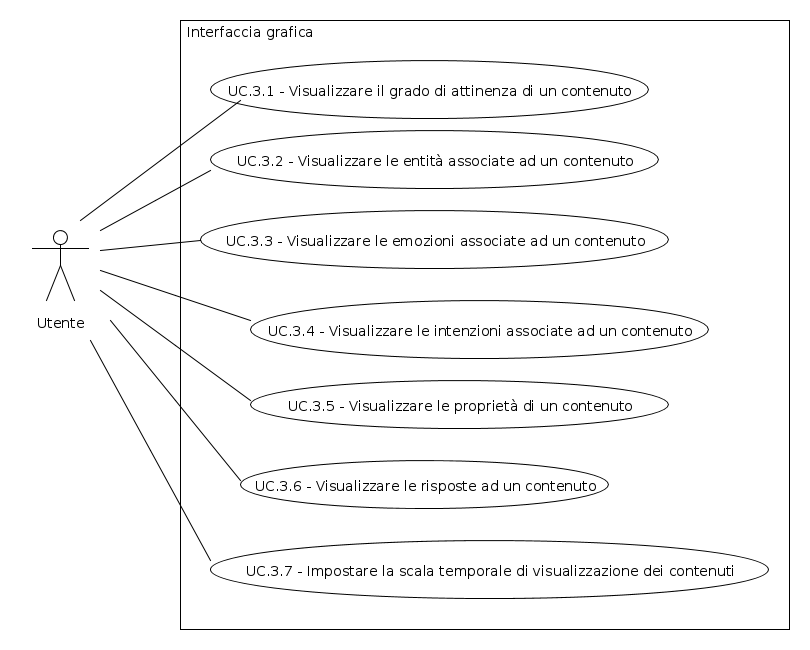
\includegraphics[width=12cm]{uc_3.png}
			\label{gfx:uc:3}
			\caption{UC.3 - Consultazione dei risultati di ricerca}
		\end{center}
	\end{figure}

	Il diagramma dei casi d'uso descrive le modalità di consultazione dei contenuti individuati dalla ricerca, delle relative informazioni e delle reciproche relazioni.

	\subsection[UC.3.1]{UC.3.1 - Visualizzare il grado di attinenza di un contenuto}
	\label{sec:stage:ar:uc:3_1}
	\paragraph{Attori:}
	\paragraph{Precondizioni:} il sistema visualizza i contenuti corrispondenti ai criteri di ricerca immessi e ai filtri impostati.
	\paragraph{Postcondizioni:} il sistema visualizza graficamente il grado di attinenza rispetto ai criteri di ricerca.
	\paragraph{Scenario principale} \hfill \\
	L'utente seleziona un contenuto incluso tra i risultati di ricerca.

	\subsection[UC.3.2]{UC.3.2 - Visualizzare le entità associate ad un contenuto}
	\label{sec:stage:ar:uc:3_2}
	\paragraph{Attori:} utente
	\paragraph{Precondizioni:} il sistema visualizza i contenuti corrispondenti ai criteri di ricerca immessi e ai filtri impostati.
	\paragraph{Postcondizioni:} il sistema mostra l'elenco delle entità associate al contenuto selezionato evidenziando quelle corrispondenti ai criteri di ricerca.
	\paragraph{Scenario principale} \hfill \\
	L'utente seleziona un contenuto incluso tra i risultati di ricerca e apre la lista delle entità.

	\subsection[UC.3.3]{UC.3.3 - Visualizzare le emozioni associate ad un contenuto}
	\label{sec:stage:ar:uc:3_3}
	\paragraph{Attori:} utente
	\paragraph{Precondizioni:} il sistema visualizza i contenuti corrispondenti ai criteri di ricerca immessi e ai filtri impostati.
	\paragraph{Postcondizioni:} il sistema mostra l'elenco delle emozioni associate al contenuto selezionato.
	\paragraph{Scenario principale} \hfill \\
	L'utente seleziona un contenuto incluso tra i risultati di ricerca e apre la lista delle emozioni.

	\subsection[UC.3.4]{UC.3.4 - Visualizzare le intenzioni associate ad un contenuto}
	\label{sec:stage:ar:uc:3_4}
	\paragraph{Attori:} utente
	\paragraph{Precondizioni:} il sistema visualizza i contenuti corrispondenti ai criteri di ricerca immessi e ai filtri impostati.
	\paragraph{Postcondizioni:} il sistema mostra l'elenco delle intenzioni associate al contenuto selezionato.
	\paragraph{Scenario principale} \hfill \\
	L'utente seleziona un contenuto incluso tra i risultati di ricerca e apre la lista delle intenzioni.

	\subsection[UC.3.5]{UC.3.5 - Visualizzare le proprietà di un contenuto}
	\label{sec:stage:ar:uc:3_5}
	\paragraph{Attori:} utente
	\paragraph{Precondizioni:} il sistema visualizza i contenuti corrispondenti ai criteri di ricerca immessi e ai filtri impostati.
	\paragraph{Postcondizioni:} il sistema visualizza le proprietà del contenuto selezionato. 
	\paragraph{Scenario principale} \hfill \\
	L'utente seleziona un contenuto incluso tra i risultati di ricerca ed apre la scheda delle proprietà:
	\begin{itemize}
	\item argomento;
	\item autore;
	\item data di pubblicazione;
	\item giudizio;
	\item tipo;
	\item titolo.
	\end{itemize}

	\subsection[UC.3.6]{UC.3.6 - Visualizzare le risposte ad un contenuto}
	\label{sec:stage:ar:uc:3_6}
	\paragraph{Attori:} utente
	\paragraph{Precondizioni:} il sistema visualizza i contenuti corrispondenti ai criteri di ricerca immessi e ai filtri impostati.
	\paragraph{Postcondizioni:} il sistema visualizza separatamente dai risultati di ricerca la discussione generata dal contenuto selezionato.
	\paragraph{Scenario principale}
	\begin{enumerate}
	\item l'utente seleziona un contenuto incluso tra i risultati di ricerca visualizzati;
	\item l'utente apre la prospettiva discussione.
	\end{enumerate}

	\subsection[UC.3.7]{UC.3.8 - Impostare la scala temporale di visualizzazione dei contenuti}
	\label{sec:stage:ar:uc:3_}
	\paragraph{Attori:} utente
	\paragraph{Precondizioni:} il sistema visualizza i contenuti corrispondenti ai criteri di ricerca immessi e ai filtri impostati in ordine temporale.
	\paragraph{Postcondizioni:} il sistema aggiorna la visualizzazione secondo l'unità temporale specificata.
	\paragraph{Scenario principale}
	L'utente esprime la scala temporale desiderata in una delle seguenti unità di misura:
	\begin{itemize}
	\item giorni;
	\item settimane;
	\item mesi;
	\item anni.
	\end{itemize}
	oppure seleziona la regolazione automatica (basata sulle date di pubblicazione dei contenuti visualizzati).
	\paragraph{Scenari alternativi}
	\begin{enumerate}
	\item L'utente inserisce un valore negativo o non intero
		\begin{enumerate}
		\item Il sistema restituisce un messaggio di errore e ripristina il valore precedente;
		\item l'utente può inserire un valore corretto.
		\end{enumerate}
	\end{enumerate}

	% SECTION
	\section{UC.4 - Gestione dei filtri utente}
	\label{ch:stage:ar:uc:4}

	\begin{figure}[ht]
		\begin{center}
	    	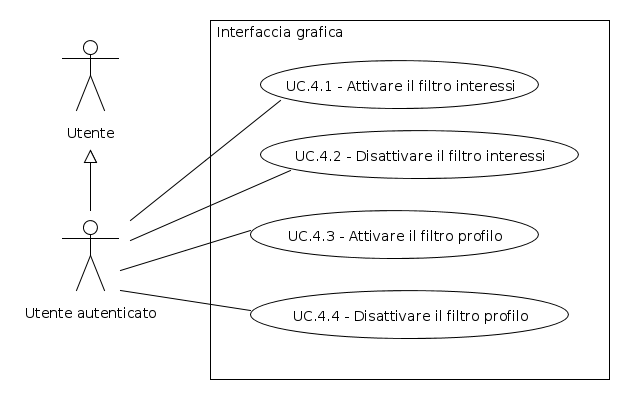
\includegraphics[width=12cm]{uc_4.png}
			\label{gfx:uc:4}
			\caption{UC.4 - Gestione dei filtri utente}
		\end{center}
	\end{figure}

	Il diagramma dei casi d'uso mostra le opzioni disponibili per l'utente autenticato riguardanti la personalizzazione della ricerca in base agli interessi e al tipo di profilo.

	\subsection[UC.4.1]{UC.4.1 - Attivare il filtro interessi}
	\label{sec:stage:ar:uc:4_1}
	\paragraph{Attori:} utente autenticato
	\paragraph{Precondizioni:} il sistema visualizza i contenuti corrispondenti ai criteri di ricerca immessi e ai filtri impostati.
	\paragraph{Postcondizioni:} il sistema omette dai risultati di ricerca i contenuti non attinenti agli interessi dell'utente.
	\paragraph{Scenario principale} \hfill \\
	L'utente disattiva il filtro basato sugli interessi.

	\subsection[UC.4.2]{UC.4.2 - Disattivare il filtro interessi}
	\label{sec:stage:ar:uc:4_2}
	\paragraph{Attori:} utente autenticato
	\paragraph{Precondizioni:} il sistema visualizza i contenuti corrispondenti ai criteri di ricerca immessi, ai filtri impostati e agli interessi dell'utente.
	\paragraph{Postcondizioni:} il sistema visualizza i contenuti corrispondenti ai criteri di ricerca immessi e ai filtri impostati, a prescindere dagli interessi dell'utente.
	\paragraph{Scenario principale} \hfill \\
	L'utente attiva il filtro basato sugli interessi.

	\subsection[UC.4.3]{UC.4.3 - Attivare il filtro profilo}
	\label{sec:stage:ar:uc:4_3}
	\paragraph{Attori:} utente autenticato
	\paragraph{Precondizioni:} il sistema visualizza i contenuti corrispondenti ai criteri di ricerca immessi e ai filtri impostati.
	\paragraph{Postcondizioni:} il sistema omette dai risultati di ricerca i contenuti non coerenti con il profilo dell'utente.
	\paragraph{Scenario principale} \hfill \\
	L'utente attiva il filtro basato sul profilo.

	\subsection[UC.4.4]{UC.4.4 - Disattivare il filtro profilo}
	\label{sec:stage:ar:uc:4_4}
	\paragraph{Attori:} utente autenticato
	\paragraph{Precondizioni:} il sistema visualizza i contenuti corrispondenti ai criteri di ricerca immessi, ai filtri impostati e al tipo di profilo dell'utente.
	\paragraph{Postcondizioni:} il sistema visualizza i contenuti corrispondenti ai criteri di ricerca immessi e ai filtri impostati, a prescindere dal tipo di profilo dell'utente.
	\paragraph{Scenario principale} \hfill \\
	L'utente disattiva il filtro basato sul profilo.

	\chapter{Requisiti}
	\label{ch:stage:ar:requisiti}

	In questo capitolo sono illustrati i requisiti del sistema software, classificati in:
	\begin{itemize}
	\item \textsc{obbligatori}: si tratta di requisiti il cui soddisfacimento è indispensabile per il corretto funzionamento del sistema;
	\item \textsc{desiderabili}: si tratta di requisiti il cui soddisfacimento conferisce un valore aggiunto al prodotto. 
	\end{itemize}

	\section{Requisiti funzionali obbligatori}
	\label{ch:stage:ar:requisiti:ob}

	\paragraph{RF.ob.1} Il sistema deve permettere l'inserimento di termini di ricerca multipli.

	\paragraph{RF.ob.2} Il sistema dev'essere in grado di riconoscere le etichette inserite.

	\paragraph{RF.ob.3} Il sistema dev'essere in grado di elencare le accezioni di un'etichetta.

	\paragraph{RF.ob.4} Il sistema deve permettere di selezionare un'accezione di un'etichetta inserita.

	\paragraph{RF.ob.5} Il sistema deve permettere di restringere l'ambito di ricerca a etichette o frasi.

	\paragraph{RF.ob.6} Il sistema deve mostrare le entità riferite dalle etichette cercate.

	\paragraph{RF.ob.7} Il sistema deve mostrare le informazioni essenziali di un'entità.

	\paragraph{RF.ob.8} Il sistema deve permettere di visualizzare la descrizione di un'entità.

	\paragraph{RF.ob.9} Il sistema deve permettere di visualizzare i padri di un'entità.

	\paragraph{RF.ob.10} Il sistema deve permettere di visualizzare i figli di un'entità.

	\paragraph{RF.ob.11} Il sistema deve permettere di sostituire un'entità con un padre.

	\paragraph{RF.ob.12} Il sistema deve permettere di sostituire un'entità con un figlio.

	\paragraph{RF.ob.13} Il sistema deve permettere di eliminare un'entità dai criteri di ricerca.

	\paragraph{RF.ob.14} Il sistema deve permettere di applicare dei filtri di raffinamento della ricerca.

	\paragraph{RF.ob.15} Il sistema deve applicare i filtri sui contenuti corrispondenti ai criteri di ricerca.

	\paragraph{RF.ob.16} Il sistema dev'essere in grado di aggiornare in tempo reale i risultati della ricerca in accordo alle entità e ai filtri.

	\paragraph{RF.ob.17} Il sistema deve permettere di visualizzare la lista degli utenti autorizzati.

	\paragraph{RF.ob.18} Il sistema deve permettere di visualizzare la lista degli utenti bloccati.

	\paragraph{RF.ob.19} Il sistema deve permettere di autorizzare un utente bloccato.

	\paragraph{RF.ob.20} Il sistema deve permettere di bloccare un utente autorizzato.

	\paragraph{RF.ob.21} Il sistema deve mostrare solo i contenuti pubblicati da utenti autorizzati.

	\paragraph{RF.ob.22} Il sistema deve permettere di visualizzare la lista dei tipi di contenuto autorizzati.

	\paragraph{RF.ob.23} Il sistema deve permettere di visualizzare la lista dei tipi di contenuto bloccati.

	\paragraph{RF.ob.24} Il sistema deve permettere di autorizzare un tipo di contenuti bloccato.

	\paragraph{RF.ob.25} Il sistema deve permettere di bloccare un tipo di contenuto autorizzato.

	\paragraph{RF.ob.26} Il sistema deve mostrare solo i contenuti il cui tipo sia autorizzato.

	\paragraph{RF.ob.27} Il sistema deve permettere di mostrare i soli contenuti pubblicati prima di una certa data.

	\paragraph{RF.ob.28} Il sistema deve permettere di mostrare i soli contenuti pubblicati oltre una certa data.

	\paragraph{RF.ob.29} Il sistema deve permettere di mostrare i soli contenuti pubblicati in una certa data.

	\paragraph{RF.ob.30} Il sistema deve permettere di mostrare i contenuti pubblicati in qualsiasi data.

	\paragraph{RF.ob.31} Il sistema deve permettere di visualizzare la lista degli argomenti autorizzati.

	\paragraph{RF.ob.32} Il sistema deve permettere di visualizzare la lista degli argomenti bloccati.

	\paragraph{RF.ob.33} Il sistema deve permettere di autorizzare un argomento bloccato.

	\paragraph{RF.ob.34} Il sistema deve permettere di bloccare un argomento autorizzato.

	\paragraph{RF.ob.35} Il sistema deve mostrare solo i contenuti relativi agli argomenti autorizzati.

	\paragraph{RF.ob.36} Il sistema deve permettere di visualizzare la lista delle emozioni autorizzate.

	\paragraph{RF.ob.37} Il sistema deve permettere di visualizzare la lista delle emozioni bloccate.

	\paragraph{RF.ob.38} Il sistema deve permettere di autorizzare un'emozione bloccata.

	\paragraph{RF.ob.39} Il sistema deve permettere di bloccare un'emozione autorizzata.

	\paragraph{RF.ob.40} Il sistema deve mostrare solo i contenuti cui siano associate emozioni autorizzate.

	\paragraph{RF.ob.41} Il sistema deve permettere di visualizzare la lista delle intenzioni autorizzate.

	\paragraph{RF.ob.42} Il sistema deve permettere di visualizzare la lista delle intenzioni bloccate.

	\paragraph{RF.ob.43} Il sistema deve permettere di autorizzare un'intenzione bloccata.

	\paragraph{RF.ob.44} Il sistema deve permettere di bloccare un'intenzione autorizzata.

	\paragraph{RF.ob.45} Il sistema deve mostrare solo i contenuti cui siano associate intenzioni autorizzate.

	\paragraph{RF.ob.46} Il sistema deve permettere di mostrare i soli contenuti aventi giudizio pari o superiore ad un certo valore.

	\paragraph{RF.ob.47} Il sistema deve permettere di mostrare i contenuti aventi un giudizio qualsiasi.

	\paragraph{RF.ob.48} Il sistema deve permettere di mostrare i soli contenuti aventi un livello di attinenza pari o superiore ad un certo valore.

	\paragraph{RF.ob.49} Il sistema deve permettere di mostrare i contenuti aventi un livello di attinenza qualsiasi.

	\paragraph{RF.ob.50} Il sistema deve visualizzare i contenuti informativi corrispondenti ai criteri di ricerca e ai filtri impostati.

	\paragraph{RF.ob.51} Il sistema deve mostrare il grado di attinenza di un contenuto informativo rispetto ai criteri di ricerca.

	\paragraph{RF.ob.52} Il sistema dev'essere in grado di mostrare le entità assegnate al contenuto.

	\paragraph{RF.ob.53} Il sistema dev'essere in grado di evidenziare quali tra le entità cercate siano assegnate al contenuto.

	\paragraph{RF.ob.54} Il sistema dev'essere in grado di mostrare le emozioni assegnate al contenuto.

	\paragraph{RF.ob.55} Il sistema dev'essere in grado di mostrare le intenzioni assegnate al contenuto.

	\paragraph{RF.ob.56} Il sistema deve mostrare le proprietà di un contenuto informativo.

	\paragraph{RF.ob.57} Il sistema deve permettere di selezionare un contenuto informativo.

	\paragraph{RF.ob.58} Il sistema deve mostrare le relazioni esistenti tra i contenuti.

	\paragraph{RF.ob.59} Il sistema deve permettere di visualizzare separatamente la discussione generata da un contenuto informativo.

	\paragraph{RF.ob.60} Il sistema deve evidenziare i contenuti informativi della discussione non attinenti ai criteri di ricerca.

	\paragraph{RF.ob.61} Il sistema deve visualizzare i contenuti in un piano temporale.

	\paragraph{RF.ob.62} Il sistema deve regolare automaticamente la scala del piano temporale in base alle date di pubblicazione dei contenuti.

	\paragraph{RF.ob.63} Il sistema deve permettere di regolare la scala temporale.

	\paragraph{RF.ob.64} Il sistema deve mostrare il numero di contenuti disponibili per ogni unità temporale.

	\section{Requisiti funzionali desiderabili}
	\label{ch:stage:ar:requisiti:op}

	\paragraph{RF.de.1} Il sistema deve filtrare automaticamente i risultati in base agli interessi dell'utente registrato

	\paragraph{RF.de.2} Il sistema deve consentire di disabilitare il filtro dei risultati di ricerca basato sugli interessi dell'utente

	\paragraph{RF.de.3} Il sistema deve consentire di abilitare il filtro dei risultati di ricerca basato sugli interessi dell'utente

	\paragraph{RF.de.4} Il sistema deve filtrare automaticamente i risultati in base al profilo di esperienza dell'utente registrato

	\paragraph{RF.de.5} Il sistema deve consentire di disabilitare il filtro dei risultati di ricerca basato sul profilo di esperienza dell'utente

	\paragraph{RF.de.6} Il sistema deve consentire di abilitare il filtro dei risultati di ricerca basato sul profilo di esperienza dell'utente

	\section{Tracciamento dei requisiti}
	\label{ch:stage:ar:requisiti:matrice}
	Il tracciamento di requisiti e casi d'uso è consultabile nel foglio elettronico \textit{tracciamento.ods}, allegato alla presente documentazione.

\end{document}
